\graphicspath{{results/fig/}}

\chapter{Results}
\label{chap:results}
An incremental approach to testing was done for this project. Each software component was tested individually. This section will report on the results of the incremental testing as well as the results of the entire system. Lastly the noise extraction module will be used to calculate the mean square flux noise figure of an actual SQUID design with measured mean square flux noise values.
\section{The GMSH extraction module}

\subsection{Test setup}
\subsection{Results}

\section{The mesh optimisation module}

\subsection{Test setup}
\subsection{Results}

\section{The noise extraction module}
This module was tested by comparing analytic solutions to numerical results for 2 different geometric setups. The first geometry is a thin wire with diameter $D$ and loop radius $R$. The second is a thin film circular loop of loop radius $R$ and track width $W$. The module is further tested by performing the noise analysis on a real SQUID design.
\subsection{Test setup}
\subsubsection*{The wire loop}
Equation \ref{eq:MSFNfinal} describes the analytical solution for a thin wire loop. The assumption made in the derivation of this equation is that $R >> D$. The test is performed was a parameter sweep from $R = \si{8}{\mu m}$ and $D = \si{5}{\mu m}$ to $R = \si{45}{\mu m}$ and $D = \si{0.4}{\mu m}$ as shown figure \ref{fig:meshedTorus}. The parameter sweep was automated using a python script.

\begin{figure}[h]
    \centering
    \begin{subfigure}[b]{0.45\textwidth}
        \centering
        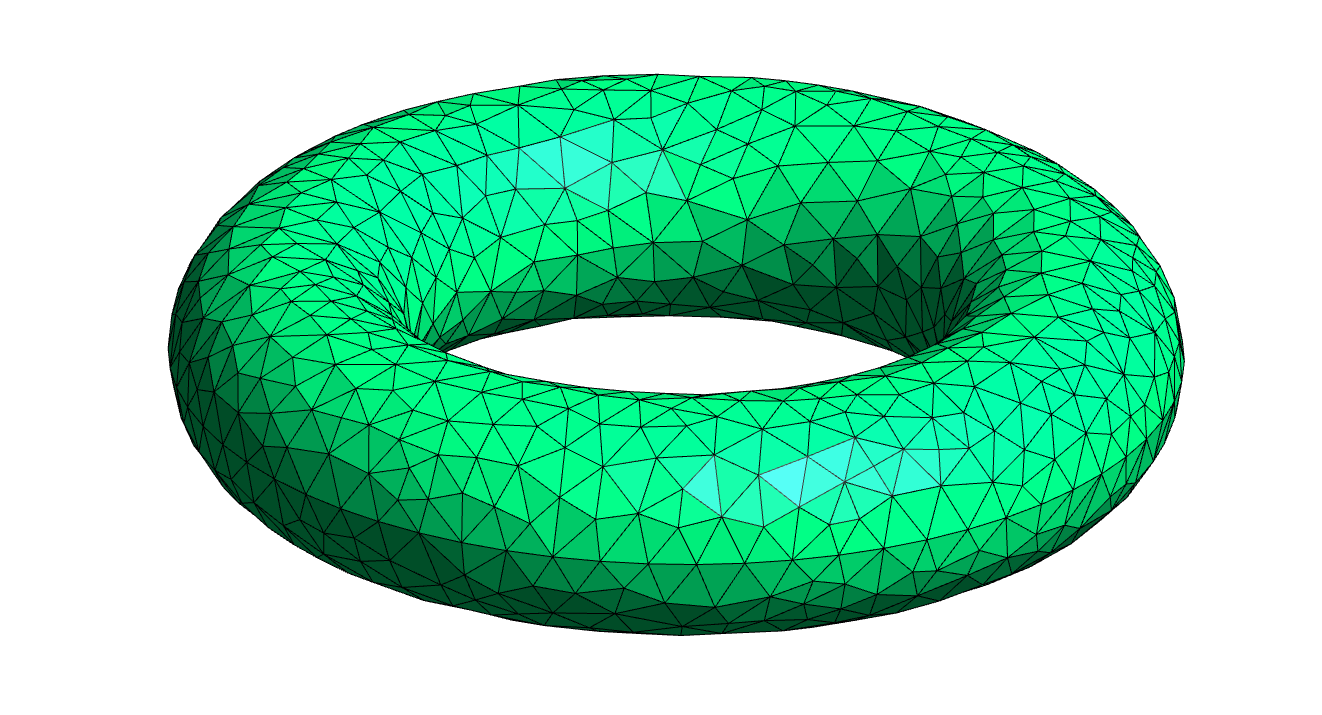
\includegraphics[width=0.5\textwidth]{torusThick}
        \caption{The meshed torus with the smallest loop radius and largest wire diameter}
    \end{subfigure}
    \hfill
    \begin{subfigure}[b]{0.45\textwidth}
        \centering
        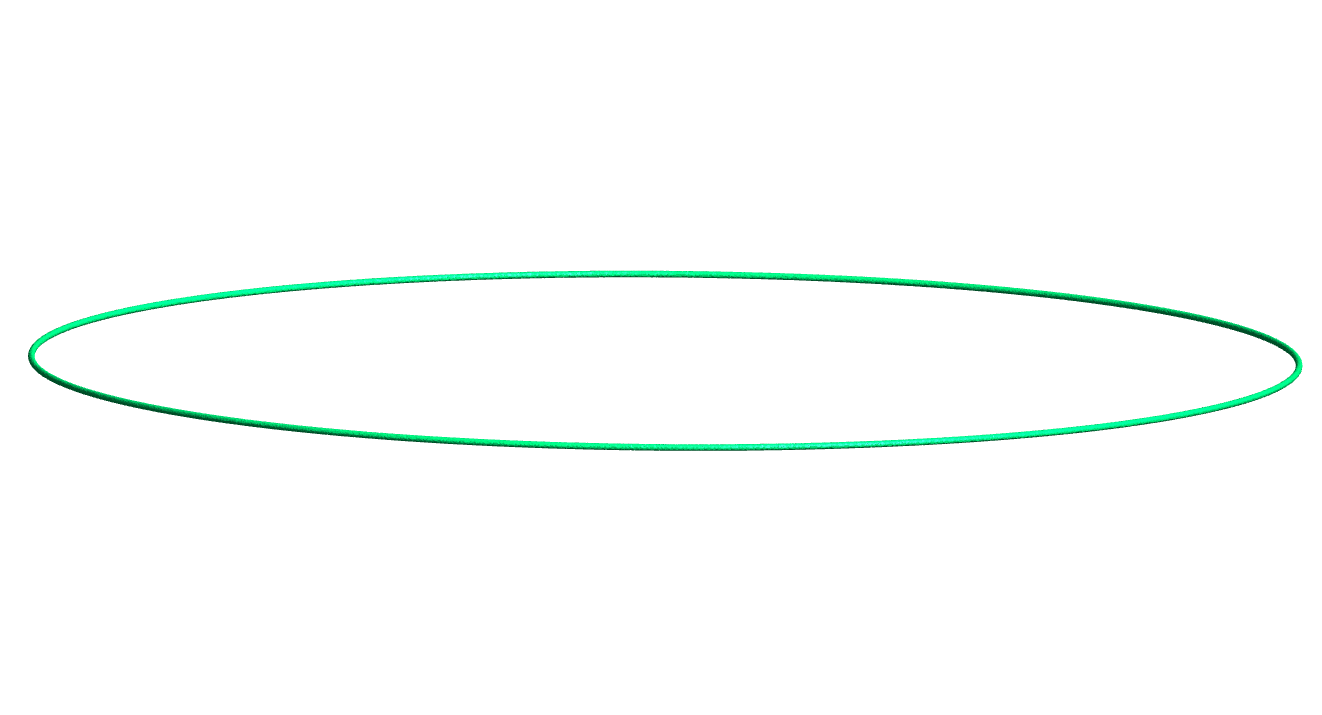
\includegraphics[width=0.5\textwidth]{torusThin}
        \caption{The meshed torus with the largest loop radius and smallest wire diameter}
    \end{subfigure}
    \caption{A figure showing the two extremes of the parameter sweep for a torus. The images show the surface mesh as generated by GMSH.}
    \label{fig:meshedTorus}
\end{figure}
\subsection{Results}

\subsubsection*{The wire loop}
The results of the parameter sweep are summarized in figure \ref{fig:resTorus}.
\begin{figure}[H]
    \centering
    \begin{subfigure}[b]{0.48\textwidth}
        \centering
        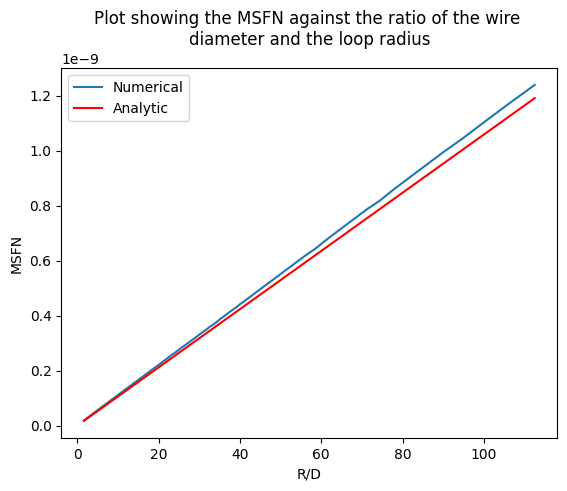
\includegraphics[width=\textwidth]{torusAVN}
        \caption{The meshed torus with the smallest loop radius and largest wire diameter}
        \label{fig:MSFNvRD}
    \end{subfigure}
    \hfill
    \begin{subfigure}[b]{0.48\textwidth}
        \centering
        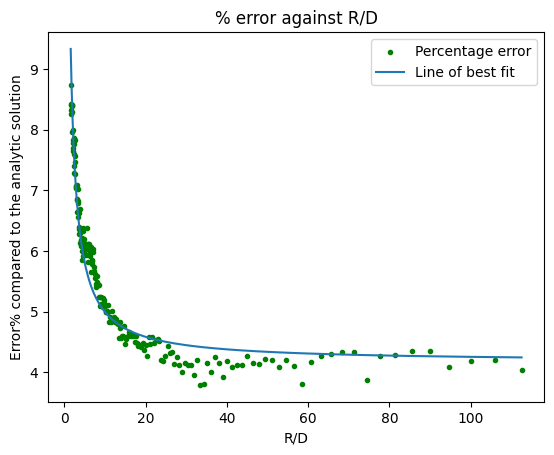
\includegraphics[width=\textwidth]{torusEVRD}
        \caption{The meshed torus with the largest loop radius and smallest wire diameter}
        \label{fig:evRD}
    \end{subfigure}
    \caption{A figure showing the two extremes of the parameter sweep for a torus. The images show the surface mesh as generated by GMSH.}
    \label{fig:resTorus}
\end{figure}
From figure \ref{fig:resTorus} it is clear to see that the relative percentage error compared to the analytic solution decreases as the ration of the loop radius to diameter increases. This behaviour can be attributed to the assumption: $R >> D$. The decrease in error clearly demonstrates that the noise extraction module works for this particular setup. In figure \ref{fig:MSFNvRD} the analytical and numerical results increase linearly with an increase in $\frac{R}{D}$ as expected.
Additional tests where performed to analyse the performance of the noise extraction module as well as the effect of using a surface mesh to calculate the current density. \textcolor{red}{Insert triangle vs tet comparison here}